
\documentclass{llncs}
\usepackage{graphicx}        % standard LaTeX graphics tool
                             % when including figure files
\usepackage{url}
%%%%%%%%%%%%%%%%%%%%%%%%%%%%%%%%%%%%%%%%%%%%%%%%%%%%%%%%%%%%%%%%%%%%%%%%%%%%%%%%%%%%%%%%%
\usepackage{subfigure}
\begin{document}
\sloppy

\title{Increasing User Engagement in a Volunteer-Based Ephemeral Evolutionary Computation System}
\titlerunning{Increasing Engagement in a Volunteer-Based Ephemeral Evolutionary Computation System}


\author{Mario Garc\'ia-Valdez\inst{1} \and Juan J. Merelo Guerv\'os\inst{2} \and  Lucero Lara \inst{1}}

\institute{Instituto Tecnol\'ogico de Tijuana, Tijuana BC, Mexico
\and
Universidad de Granada, Granada, Spain
\email{mario@tectijuana.edu.mx}\\
\email{jmerelo@geneura.ugr.es}}

\authorrunning{Garc\'ia-Valdez, Merelo, \& Lara }

\maketitle


\begin{abstract}

One way of creating distributed computing system is to use volunteers who
provide their own computing resources or storage to contribute to a common effort.
By runnning a script in a web page, collaboration is straightforward, but also ephemeral.
Resources depend on the amount of time a user lends, whicn means that 
the user has to be kept engaged to obtain as many computing cycles as
possible. In this paper, we analyze a volunteer-based evolutionary computing system called
NodIO with the objective of discovering rules that encourage volunteer
participation thus increasing the overall computing power. We present the results of
an experiment where a gammification technique is applied by adding a leaderboard 
showing the top scores achieved by registered contributors. In the NodIO system volunteers can
participate without the need to create an account, so the question was
if the need to register would have a negative impact on user participation. 
The experiment results show that even if only a small percentege of users created an account,
those participating in the competition provided around 90\%.

\keywords{Distributed Evolutionary Algorithms, Volunteer Computing}
\end{abstract}

\begin{figure*}[t]
    \centering
        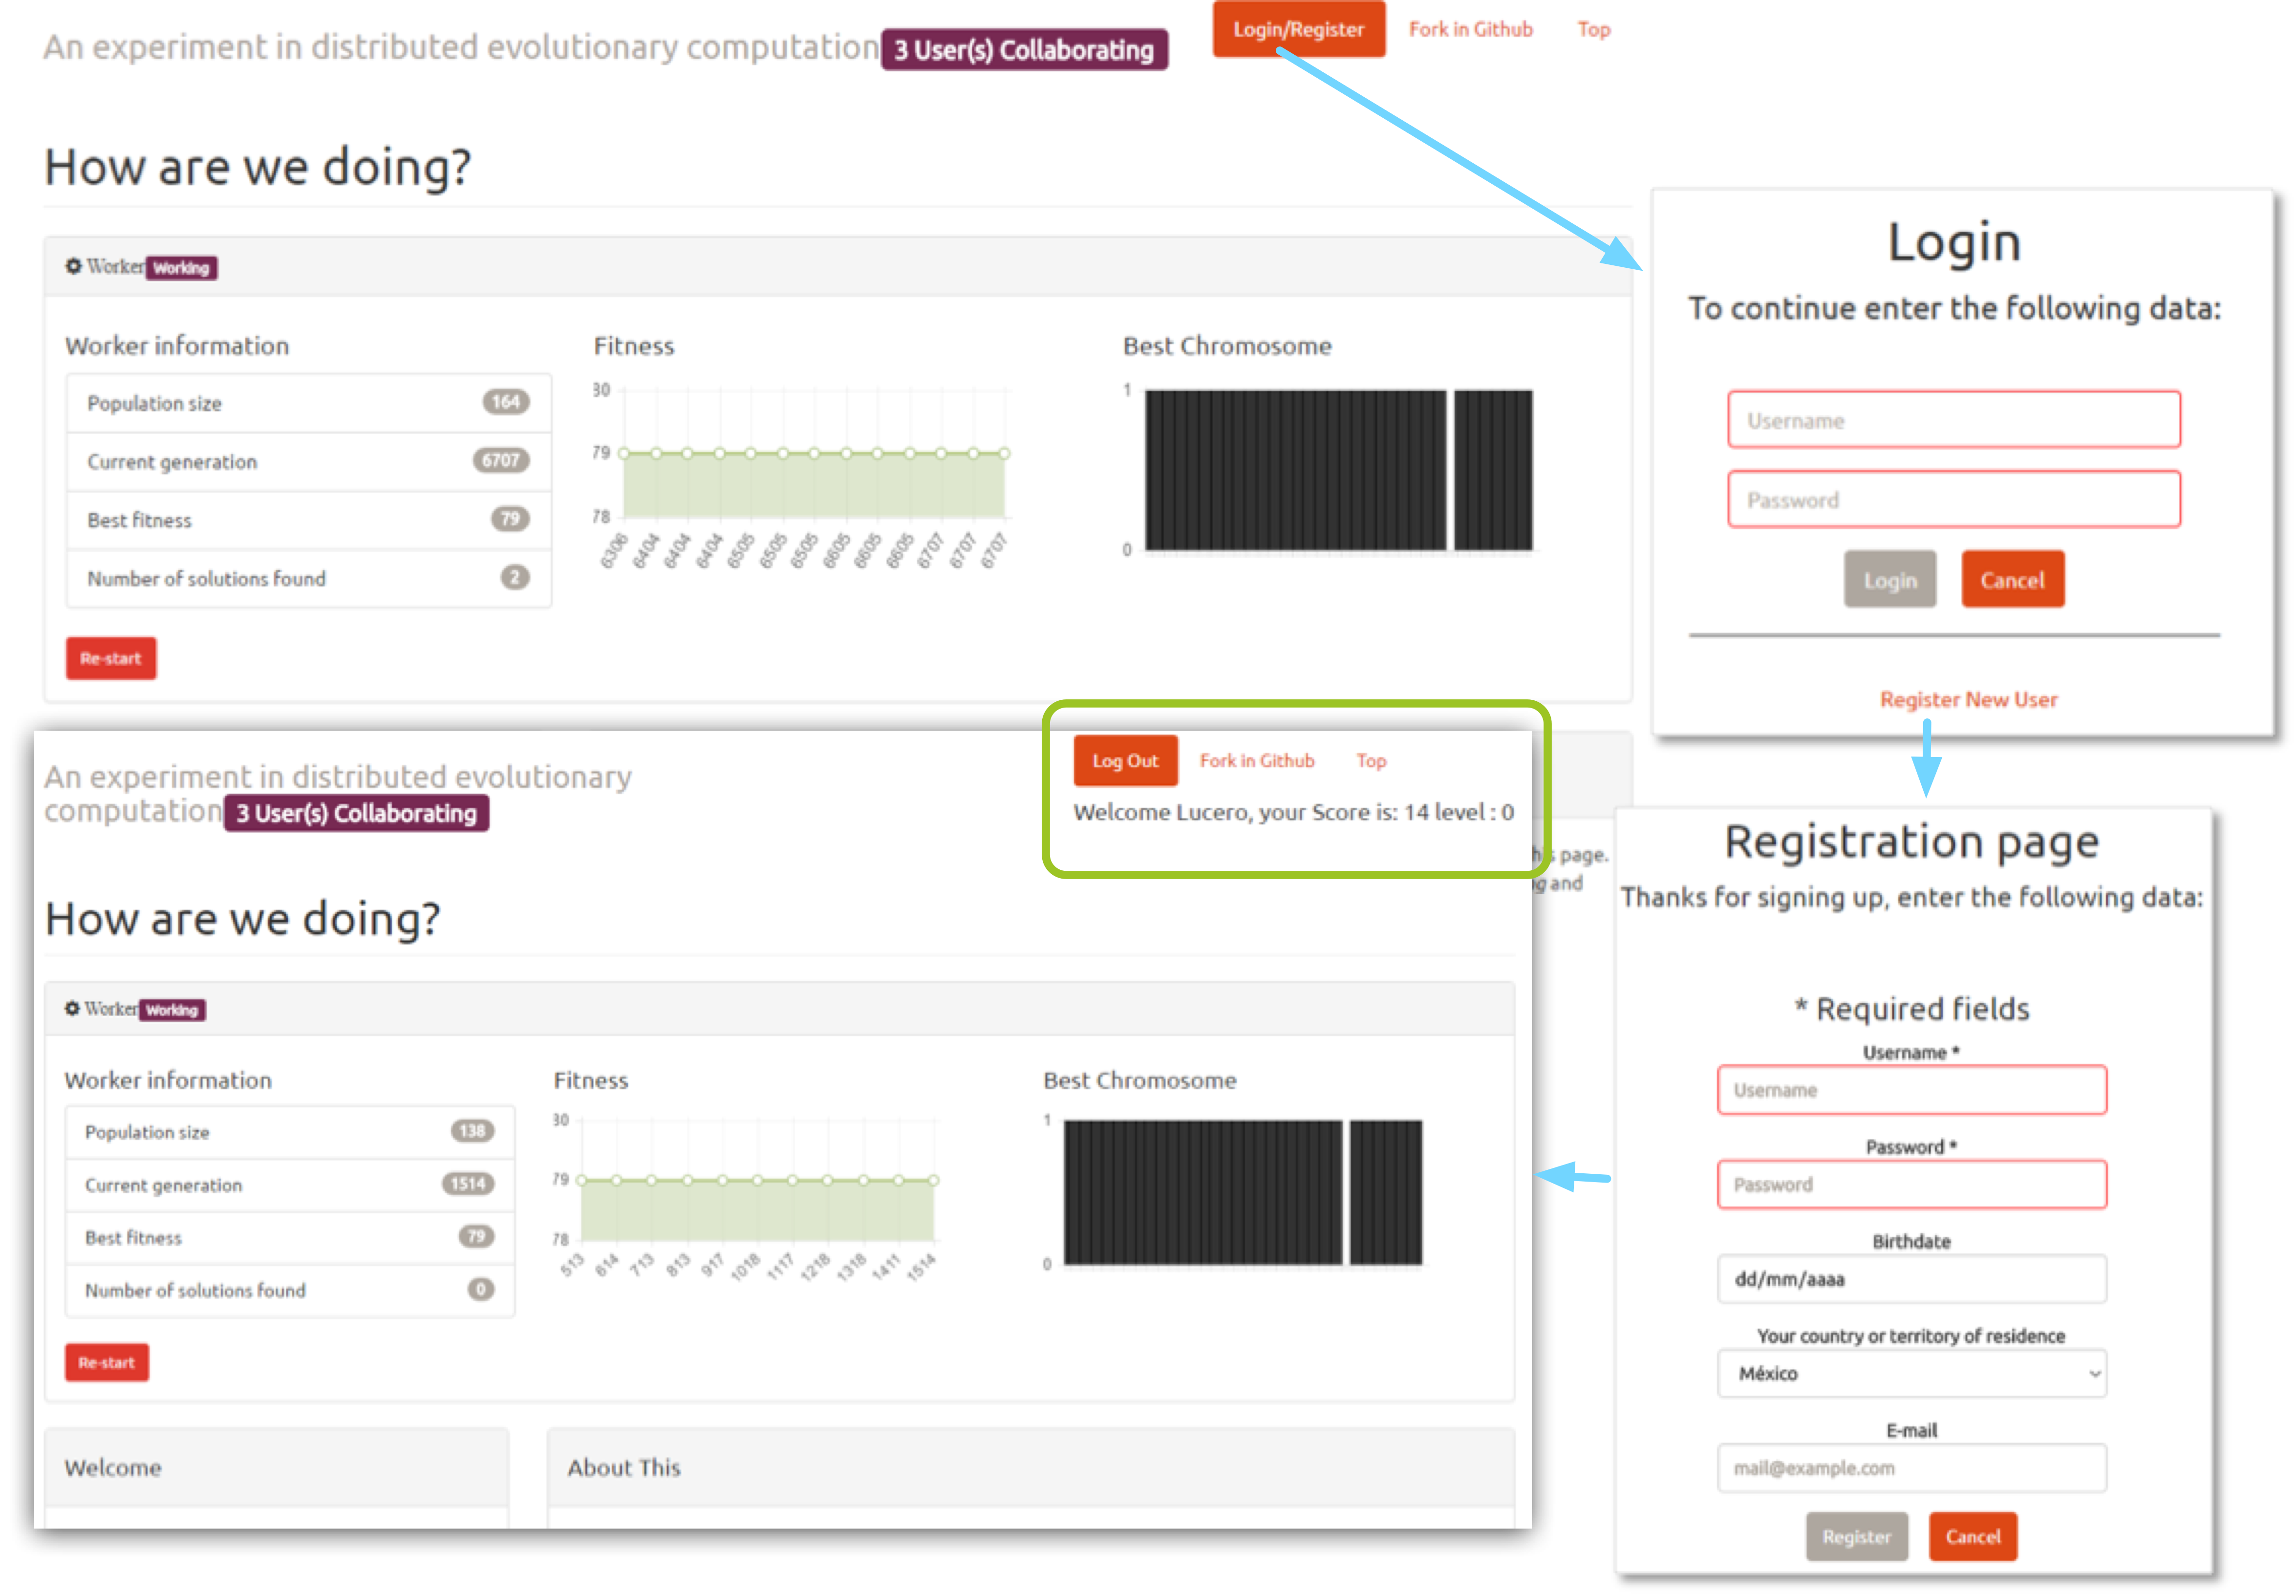
\includegraphics[width=5in]{img/login.png}
    \caption{Comparison of 30 runs of the 128 Bit OneMax problem. 
    Box-plot of the number of evaluations needed for solution, with a 2, 6 and 12 workers
    homogeneous configuration on the left side, and Heterogeneous configuration on the
    right side of each.
    }
    \label{fig:comp-onemax}
\end{figure*}

\section{Experiments}
\label{sec:experiments}

\subsection{Results}
\label{sec:results}

\begin{figure*}[t]
    \centering
    \subfigure  [6 workers]
    {
        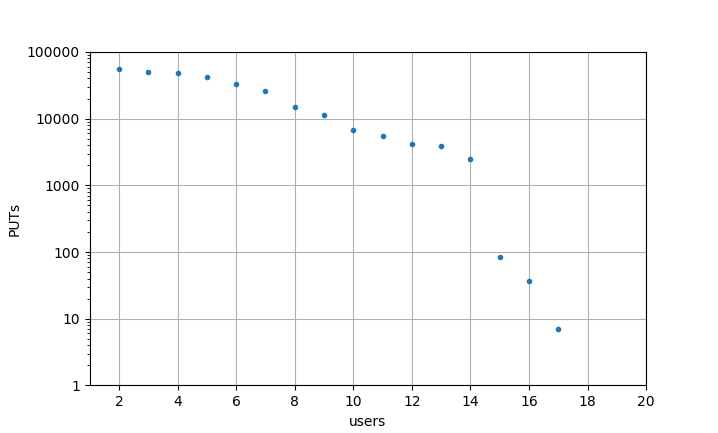
\includegraphics[width=4in]{img/puts_user.png}
    }
    \subfigure  [12 workers]
    {
        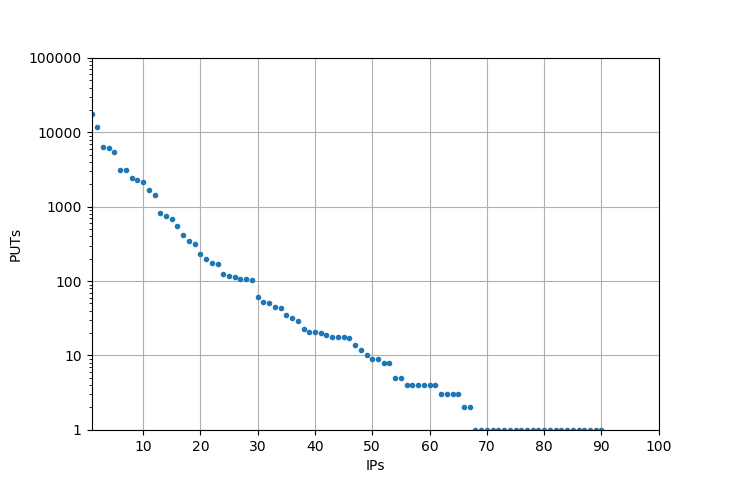
\includegraphics[width=4in]{img/puts_ip.png}
    }

    \caption{100 experiments with random parameters for the 128 Bit Griewank 
    single-objective optimization test function. Experiments are ranked by 
    the mean time to solution of 5 runs, with (a) 6 workers, and (b) 12 workers.}
    \label{fig:griewank}
\end{figure*}


\begin{figure*}[t]
    \centering
        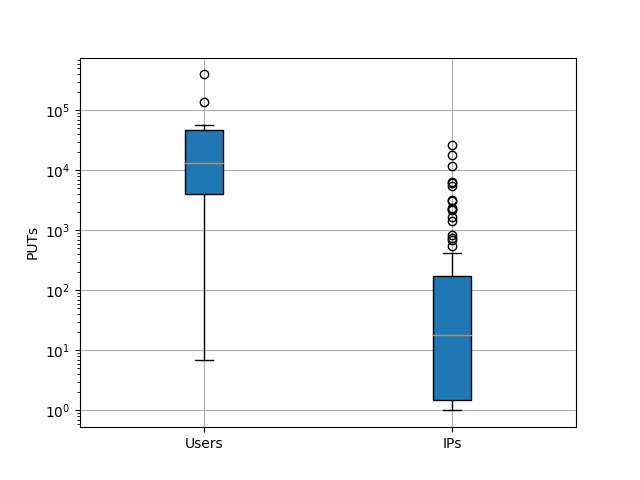
\includegraphics[width=4in]{img/puts_box.png}
    \caption{Comparison of 30 runs of the 128 Bit OneMax problem. 
    Box-plot of the number of evaluations needed for solution, with a 2, 6 and 12 workers
    homogeneous configuration on the left side, and Heterogeneous configuration on the
    right side of each.
    }
    \label{fig:comp-onemax}
\end{figure*}

\begin{figure*}[t]
    \centering
        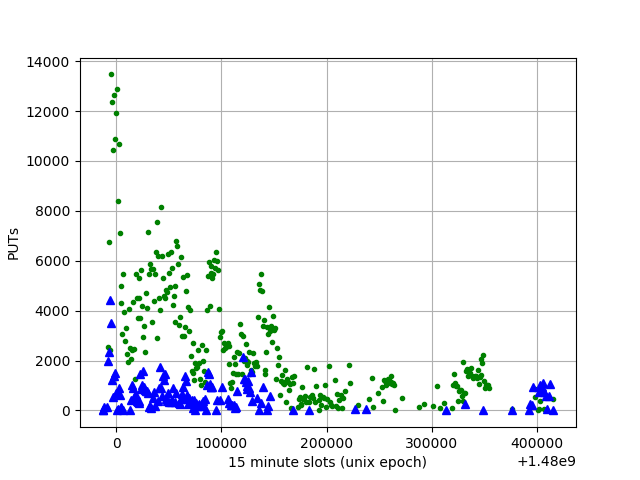
\includegraphics[width=5in]{img/puts_by_time.png}
    \caption{Comparison of 30 runs of the 128 Bit OneMax problem. 
    Box-plot of the number of evaluations needed for solution, with a 2, 6 and 12 workers
    homogeneous configuration on the left side, and Heterogeneous configuration on the
    right side of each.
    }
    \label{fig:comp-onemax}
\end{figure*}
\begin{figure*}[t]
    \centering
        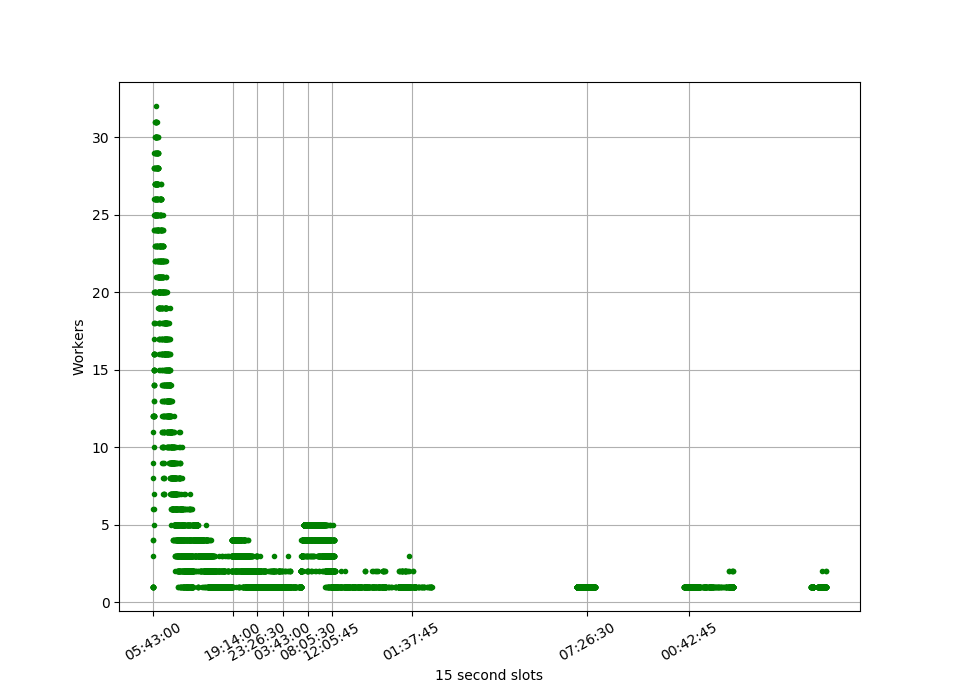
\includegraphics[width=5in]{img/workers_best_user.png}
    \caption{Comparison of 30 runs of the 128 Bit OneMax problem. 
    Box-plot of the number of evaluations needed for solution, with a 2, 6 and 12 workers
    homogeneous configuration on the left side, and Heterogeneous configuration on the
    right side of each.
    }
    \label{fig:comp-onemax}
\end{figure*}
\begin{figure*}[t]
    \centering
        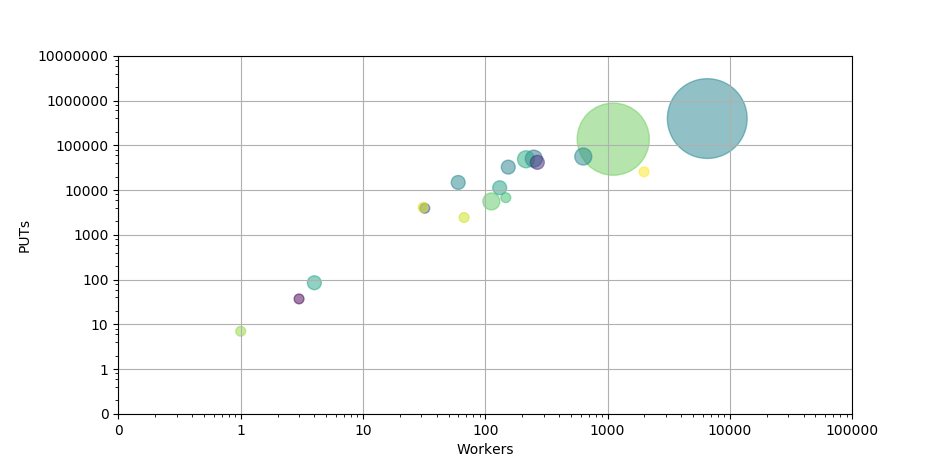
\includegraphics[width=5in]{img/workers_put_ip.png}
    \caption{Comparison of 30 runs of the 128 Bit OneMax problem. 
    Box-plot of the number of evaluations needed for solution, with a 2, 6 and 12 workers
    homogeneous configuration on the left side, and Heterogeneous configuration on the
    right side of each.
    }
    \label{fig:comp-onemax}
\end{figure*}


\end{document}
